\documentclass[fleqn,10pt]{wlpeerj}
\title{Comprehensive, structurally-curated alignment and phylogeny of vertebrate biogenic amine receptors}

\author[1,2,3]{Stephanie J. Spielman}
\author[1,2,3]{Keerthana Kumar}
\author[4,5]{Ahmad R. Sedaghat}
\author[1,2,3]{Claus O. Wilke}
\affil[1]{Department of Integrative Biology, The University of Texas at Austin, Austin, U.S.A.}
\affil[2]{Institute of Cellular and Molecular Biology, The University of Texas at Austin, Austin, U.S.A.}
\affil[3]{Center for Computational Biology and Bioinformatics, The University of Texas at Austin, Austin, U.S.A.}
\affil[4]{Department of Otolaryngology–Head and Neck Surgery, Massachusetts Eye and Ear Infirmary, Boston, Massachusetts, U.S.A.}
\affil[5]{Department of Otology and Laryngology, Harvard Medical School, Boston, Massachusetts, U.S.A.}

\keywords{biogenic amine receptors, G-protein coupled receptors, multiple sequence alignment, phylogenetics, protein evolution}


\begin{abstract}
Biogenic amine receptors play critical roles in regulating behavior and physiology, particularly within the central nervous system, in both vertebrates and invertebrates. Members of the G-protein coupled receptor (GPCR) family, these receptors interact with endogenous bioamine ligands, such as dopamine, serotonin, and epinephrine, and they are targeted by a wide array of pharmaceuticals. Despite their clear clinical and biological importance, the evolutionary history of biogenic amine receptors remains poorly characterized. In particular, the relationships among biogenic amine receptors, as well as any specific evolutionary constraints acting within distinct receptor subtypes, are largely unknown. To advance and facilitate studies in this receptor family, we have constructed a large, high-quality, structurally-curated sequence alignment of vertebrate biogenic amine receptors. Phylogenetic analysis with this comprehensive alignment offers dramatic improvements over structurally-naive alignments. Using this alignment and phylogeny, we deduce novel biogenic amine receptor relationships, identify misannotated and uncharacterized sequences, and uncover previously unrecognized lineage-specific receptor clades. We release our comprehensive alignment and its corresponding phylogeny as a resource for any research group interested in studying the dynamic evolution and sequence patterns inherent to the biogenic amine receptors.
\end{abstract}

\begin{document}

\flushbottom
\maketitle
\thispagestyle{empty}


\section*{Introduction}

Biogenic amines, such as the molecules serotonin and dopamine, play critical roles in virtually all Metazoans and exert significant influence on both behavior and physiology. In vertebrates, the biogenic amine receptor family, which includes dopamine (DRD), histamine (HRH), trace (TAAR), adrenergic (ADR), muscarinic cholinergic (mAChR), and most serotonin receptors (5HTR), primarily mediate biogenic amine activity.  Biogenic amine receptors belong to the broad family of G protein-coupled receptors (GPCRs), one of the largest and most diverse eukaryotic receptor families. Indeed, due to the extensive diversity of biological functions they direct and the ongoing expansion of their ligand repertoire, GPCRs are considered one of the most evolutionarily innovative and successful gene families \citep{BockaertPin1999,Lagerstrom2008}.

Biogenic amine receptors form a clade within the large Rhodopsin-like GPCR family \citep{Fredrikssonetal2003,KakaralaJamil2014}, whose emergence likely accompanied that of the Opisthokont (Fungi and Metazoa) lineage \citep{Krishnan2012}. The Rhodopsin-like family expanded substantially in Metazoa, and the specific diversification of biogenic amine receptors has contributed significantly to central nervous system functioning \citep{Callieretal2003,Nichols2008}. Like all GPCRs, biogenic amine receptors have a charcterisitic, highly-conserved structure of seven transmembrane (TM) domains separated by three extracellular (ECL) and three intracellular (ICL) loops, and they propagate intracellular signaling through a G protein-mediated pathway. Moreover, these receptors are prominent targets for a wide array of pharmaceuticals aimed to treat myriad diseases such as schizophrenia, migraines, hypertension, allergies and asthma, and stomach ulcers \citep{Schoneberg2004,Eversetal2005,Masonetal2012}.

In spite of these receptors' biological and clinical importance, studies on their evolution are limited and have predominantly focused on individual receptor subtypes, namely TAAR \citep{Gloriametal2005,Lindemann2005,Hashiguchi2007}, DRD \citep{Callieretal2003,Yamamotoetal2013}, and 5HTR \citep{Anbazhagan2010}. Moreover, many of these studies, and indeed studies on the general evolution of the Rhodopsin-like family, have examined very narrow species distributions, for instance specifically teleosts \citep{Gloriametal2005}, primates \citep{Anbazhagan2010}, humans and mice \citep{Vassilatis2003,KakaralaJamil2014}, or even strictly humans \citep{Fredrikssonetal2003}. Thus, virtually no studies accounting for the full breadth of vertebrate bioamine receptor sequences have been conducted.

To gain a comprehensive understanding of this receptor family's evolution, a high-quality multiple sequence alignment (MSA) is needed. MSAs provide the founation for nearly all comparative sequence analyses, and they are commonly used to locate conserved sequence motifs, identify functionally important residues, and investigate evolutionary histories. As constructing an MSA represents the first step in any sequence analysis, MSA errors are known to bias these downstream analyses \citep{Ogden2006, Wong2008, Jordan2012}. It is therefore crucial to ensure accuracy in MSAs to the extent possible. 

For GPCR sequences, in particular, any MSA should recapitulate the canonical 7TM structure, which a naive alignment of sequences cannot necessarily accomplish. While there are certain MSA software platforms that explicitly incorporate structural information into the alignment algorithm [eg.\ 3DCoffee \citep{3dcoffee} and PROMALS3D \citep{promals3d}], these programs are fairly computationally-intensive and thus ill-suited for large-scale applications. Furthermore, such programs require the use of a single crystal structure to guide sequence alignment. While all GPCRs contain seven TM domains, different GPCR subfamilies, particularly the biogenic amine receptors, feature a wide variety of ICL and ECL sizes. For example, human HRH1 and DRD3 contain roughly 27 and 117 residues, respectively, in their ECL3 domains, and roughly 68 and 14 residues, respectively, in their ICL3 domains [as predicted by GPCRHMM \citep{Wistrand2006}]. Thus, aligning diverse sequences using a single crystral structure may not effectively capture the domain variability across biogenic amine receptor subtypes. A desirable alignment strategy would instead anchor all sequences by their conserved TM domains without inappropriately constraining the heterogeneous ECL and ICL domains.

Here, we have constructed such an MSA using a novel iterative strategy to ensure that all seven TM domains aligned correctly across all sequences, thus yielding the most comprehensive (3039 sequences) and structurally-curated vertebrate biogenic amine receptor MSA to date. We used this MSA to construct a structurally-aware maximum likelihood (ML) phylogeny of vertebrate biogenic amine receptors, and we found that our structurally-curated MSA offered dramatic improvements in phylogenetic fit relative to a structurally-naive MSA. Using this structurally-aware phylogeny, we were able to discern relationships among biogenic amine receptor subtypes with a far increased level of sensitivity relative to previous studies, as well as identify novel lineage-specific receptor clades and clarify NCBI annotations for over 30 sequences. 

We present this vertebrate biogenic amine receptor MSA and its corresponding phylogeny as a resource for any group interested in studying the dynamic evolutionary processes, structural, and/or functional constraints operating within this exceptionally important GPCR clade. All data, including MSAs, phylogenies, and sequence descriptions, as well as all code used to generate these data, are freely available from \\\texttt{https://github.com/sjspielman/amine\_receptors}. We expect that these data will prove extremely useful for studying both the broad patterns governing biogenic amine receptor sequence evolution and the evolutionary trends specific to certain receptor subtypes. Further, our curated MSA should serve as a helpful resource in the ongoing development of homology models and pharmaceutical therapeutics targeting these receptors \citep{Kristiansen2004,Ishiguro2004,Eversetal2005,Masonetal2012}.




\section*{Results and Discussion}

\subsection*{Constructing a structurally-curated MSA of biogenic amine receptors}

We collected all sequences using PSI-BLAST from the RefSeq \citep{refseq} database and filtered data to exclude poor-quality sequences and/or sequences with excessive ambiguities (see \emph{Methods} for details). We additionally retained only sequences that could be unequivocally classified as GPCRs using the program GPCRHMM \citep{Wistrand2006}, leaving a total dataset of 3464 receptor sequences to align. We then built a structurally-curated MSA from these 3464 receptor protein sequences according to the iterative strategy outlined in Figure~\ref{flowchart}. 

Before aligning sequences, we again used the program GPCRHMM \citep{Wistrand2006} to assign each residue in all protein sequences to its respective structural domain (extracellular, transmembrane, or intracellular). Through a hidden markov model approach, GPCRHMM uses the remarkably-conserved GPCR structure to predict domains from a given protein sequence alone with high accuracy. Indeed, previous work has shown that GPCRHMM's domain predictions map exceptionally well to resolved Rhodopsin-like GPCR crystal structures \citep{SpielmanWilke2013}.

For each iteration of the algorithm in Figure~\ref{flowchart}, we aligned protein sequences with MAFFT \citep{mafftv7}. Using the residue domain assignments computed with GPCRHMM, we determined the consensus domain for each column in this MSA. Next, we discarded all sequences for which $\geq 5\%$ of residues did not correspond to their respective column's consensus domain. We realigned the remaining sequences with MAFFT and continued in this manner until no more sequences were discarded. Importantly, this strategy did not require any manual data filtering or visual data inspection, thus avoiding any confounding subjectivity in MSA processing. The final structurally-curated MSA contained a total of 3039 sequences, which were broadly distributed across receptor subtypes and vertebrate taxa (Figure~\ref{taxa_dist}). 

From this final MSA, we additionally created a masked MSA, in which protein residues which did not conform to their respective consensus domains were replaced with a ``?''. By masking these positions with an ambiguous character, we ensured that each MSA column strictly contained residues belonging to the same structural domain. In total, 2.69\% of all MSA positions were masked for this MSA.

Figure~\ref{domains} gives a visual representation of both the naive and structurally-curated MSAs, focusing specifically on the MSA regions containing the TM domains. Clearly, many sequences in the naive MSA do not conform to the overarching GPCR structure. Instead, many of these sequences' domains are shifted out of structural frame, leading TM domains to inappropriately align with loop domains, or vice versa, and ultimately preventing MSA columns from being truly homologous. Moreover, the mere presence of these misaligned sequences in the naive MSA introduced a substantial amount of gaps, often times within a single TM domain (notably TM1 and TM7, as seen in Figure~\ref{domains}). By removing such misaligned sequences through the strategy outlined in Figure~\ref{flowchart}, many of these gaps subsequently disppeared, leading to the alignment integrity of individual TM domains. Indeed, the naive MSA contained roughly 23\% more columns than did the structurally-curated MSAs, and the vast majority of gaps in the structurally-curated MSAs fall within the highly heterogenous N-term, C-term, and ICL3 domains. 



\subsection*{Structurally-aware MSA strongly improves phylogenetic inference}

To demonstrate the utility of analyzing biogenic amine receptors data with a structurally-curated MSA, we constructed five distinct maximum likelihood (ML) phylogenies, as detailed in Table~\ref{tab:phylo_AIC}, in RAxML. First, we built a phylogeny using an MSA, again built with MAFFT \citep{mafftv7}, comprised of the full set of 3464 receptors; in other words, this MSA was not subjected to the iterative process shown in Figure~\ref{flowchart}. As this MSA was not structurally-curated, we refer to it as the ``naive'' MSA. We additionally constructed two phylogenies each from the structural unmasked and masked MSAs. Previous work has shown that both structural and functional constraints impose differing selection pressures in TM vs.\ extramembrane (EM) domains, in turn producing distinct amino-acid frequency distributions in each domain class \citep{Tourasse2000,Stevens2001,Julenius2006,Oberai2009,SpielmanWilke2013,FranzosaXueXia2013}. As our structurally-curated MSAs allowed us to precisely identify each MSA column as either TM or EM, we can conduct far more rigorous phylogentic inference using a partitioned analysis. Therefore, for each of our two structurally-curated MSAs (masked and unmasked), we inferred two ML phylogenies: one with two partitions representing TM and EM columns and one with a single partition for the entire MSA. Importantly, such a partitioned analysis would not be possible without a structurally-curated MSA.

As assessed by AIC scores, the structurally-curated masked MSA yielded a far superior phylogeny compared to all other MSAs (Table~\ref{tab:phylo_AIC}), highlighting the benefits of analyzing GPCRs in a structurally-aware context. That the masked structural MSA produced phylogenies with substantially better fits than did the unmasked MSA underscores that any structurally-aware study must be undertaken cautiously. While partitioning the MSA based on structural domains was clearly beneficial, ensuring that each MSA column strictly contained residues belonging to the same domain was critical. Having even a few TM residues in a column assigned to the EM partition, or vice versa, strongly hindered phylogenetic fit.

The masked structural MSA's improved performance over the unmasked structural MSA additionally reveals some potential benefits to MSA filtering. Previous studies have advocated filtering putatively unreliable, as determined through MSA uncertainty measures or confidence scores, regions, columns, and/or residues to reduce error in downstream-analyses \citep{Castresana2000,Wu2012,Privman2012}. However, the utility of MSA filtering remains unclear; while some have argued that filtering improves analyses \citep{Talvera2007,Wu2012,Privman2012}, others have indicated that MSA filtering only marginally influences, or even harms, analyses \citep{Schloss2010,Jordan2012,SpielmanDawsonWilke2014}. Importantly, standard MSA filtering algorithms identify regions and/or residues to remove based on MSA uncertainty or confidence scores \citep{Castresana2000,Penn2010,Wu2012,Privman2012,SpielmanDawsonWilke2014}. 

Rather than using a standard filtering algorithm, we created our masked structural MSA by filtering residues based on biological information regarding protein structure. The resulting improvement in phylogenetic fit (Table~\ref{tab:phylo_AIC}) indicates that this masking approach effectively increased signal of structurally-homologous columns. Therefore, it appears as though residue masking based on biological information can strongly benefit phylogenetic analyses.


\subsection*{Structurally-aware phylogeny reveals unknown biogenic amine receptor relationships and clades}

Our resulting phylogeny, shown in Figure~\ref{phylogeny}, represents the most comprehensive and curated vertebrate biogenic amine receptor phylogeny to date. This tree broadly captures many known features of biogenic amine receptor evolution, in particular that these receptors do not cluster based on ligand-binding but rather have undergone extensive functional convergent evolution. Indeed, our phylogeny reveals that only two ligand-based receptor classes, mAChR and TAAR, are truly monophyletic. 

Our phylogeny features remarkably high bootstrap support for each distinct clade of receptor subtypes. We additionally find very strong support for three deeper nodes in the phylogeny that reveal the relationships among distinct receptor subtypes. The first contains the three clades HRH1, mAChR, and HRH-3,4, the second contains the clades 5HTR-1, 5HTR-5, and 5HTR-7, and the third contains the 5HTR-4 and TAAR clades. Previous studies have yielded conflicting phylogenetic placements for the 5HTR-7 clade; some have argued that 5HTR-7 is phylogenetically distinct from all other 5HTR sequences \citep{KakaralaJamil2014}, while others have found that evidence for a single clade containing 5HTR-5,7 as a sister taxa to a clade containing ADRA1 sequences \citep{Fredrikssonetal2003}. Alternatively, we find moderate-to-strong support for the 5HTR-7 clade having originated before subsequent diversification into 5HTR-5 and 5HTR-1, and we find full support showing that ADRA1 forms an entirely distinct monophyletic group outside all other vertebrate biogenic amine receptors. In addition, as previously mentioned, our phylogeny reveals that HRH-3,4 is actually single monophyletic group. While the HRH-4 clade contains strictly mammalian sequences, including monotreme (platypus) sequences, HRH-3 sequences are broadly distributed across vertebrate taxa. We therefore hypothesize that HRH-4 arose from an HRH-3 duplication concurrent with mammalian origins.

In addition, phylogeny allowed us to reclassify several misannotated and/or uncharacterized sequences (Table S1) as well as uncover an entirely unknown clade of biogenic amine receptors. This unknown clade, sister to HRH2, only contains avian sequences and a single \emph{Xenopus tropicalis} sequence. Two evolutionary scenarios may explain this taxonomic distribution: either this clade emerged concurrently with tetrapods and was secondarily lost in reptiles/birds and mammals, or this clade represents an avian-specific diversification which the \emph{Xenopus tropicalis} sequence resembles only convergently. Interestingly, the vast majority of sequences in this clade were annotated in NCBI as either octopamine or No9-like receptors, both of which are insect-specific biogenic amine receptors that do not occur in vertebrate taxa \citep{Roeder2005}. These sequence misannotations suggest an intriguing hypothesis that convergent evolution has allowed these receptors to interact with atypical ligands for vertebrates.


\subsection*{Dynamic evolution of the trace-amine associated receptors}
Of particular interest in our phylogeny are the unique evolutionary patterns revealed within the TAAR clade. While TAAR sequences do cluster together, the relationships among TAAR subtypes are highly dynamic, reflecting the extensive expansion and contraction events characterizing this receptor family's evolution \citep{Lindemann2005,Hashiguchi2007,Staubert2010,Staubert2013}. In fact, the TAAR subtree, displayed in Figure~\ref{taar_tree}, differs somewhat from previously proposed TAAR phylogenies \citep{Lindemann2005, Hashiguchi2007}. In particular, the presence of several lineage-specific subclades as well as unresolved subclades generate novel hypotheses regarding TAAR subtype origins. While TAAR-2, -3, and -4 form a well-resolved monophyly, its sister clade that contains the subtypes TAAR-5, -6, -7, -8, and -9 is less straight-forward to interpret. Indeed, the TAAR subtypes -6, -7, and -9 do not constitute distinct monophyletic groups, suggesting either poor NCBI sequence annotation or rampant diversification within this subclade. If we assume that these NCBI annotations are reasonably correct, we can deduce that this clade's ancestral sequence was most similar to TAAR-7 and subsequently diversified independently into TAAR-9 and TAAR-6, which in turn gave rise to the monophyletic TAAR-8. 

Furthermore, several lobe-finned fish (coelacanth) sequences are scattered across the TAAR tree and do not clearly cluster with any TAAR subtypes, likely reflecting this lineage's ancient divergence and unique evolutionary trajectory \citep{coelacanth2013}. The phylogenetic distribution of lobe-finned fish sequences may aid future endeavors to tease apart evolutionary origins of certain TAAR subtypes, specifically whether they represent teleost-specific duplications \citep{Gloriametal2005} or whether they represent ancient TAARs that emerged before teleost divergence but were secondarily lost in lobe-finned fish and/or tetrapods.

In addition, a small clade sister to TAAR (labeled in Figures \ref{phylogeny} and \ref{taar_tree} as TAAR$^\ast$) strictly contains sequences annotated by NCBI as ``5HTR4-like.'' At first glance, these annotations might suggest that 5HTR-4 is in fact paraphyletic, diversifying gradually before giving rise to TAARs. However, as all sequences in TAAR$^\ast$ belong taxonomically either to teleost or \emph{Xenopus tropicalis}, we suspect that this clade actually corresponds to the so-called TAAR-V cluster identified by \cite{Hashiguchi2007}. Indeed, the TAAR-V cluster contains a similar taxonomic distribution to our TAAR$^\ast$ and constitutes an outgroup to all other vertebrate TAAR sequences, as our phylogeny similarly displays.

\subsection*{Phylogenetic methods alone do not suffice to infer the evolutionary history of GPCRs}
Although we were able to identify several new features of biogenic amine receptor evolution, the majority of deeper splits in the phylogeny had very low bootstrap support. Therefore, many of the broader relationships among biogenic amine receptors remain unresolved, indicating that this phylogeny alone is not sufficient for fully resolving the relationships among biogenic amine receptors. This result highlights the limitations of using a strictly phylogenetic approach to elucidate the complex evolutionary histories of expanding gene families. Indeed, modern phylogenetic inference methods are ill-suited for deducing such relationships, particularly because MSA gaps are treated simply as missing data. In reality, gaps represent the evolutionary events of insertion and deletions (indels). Current phylogenetic methods, however, focus solely on the substitution process and ignore the evolutionary information contained in gaps, ultimately hindering phylogenetic accuracy \citep{Morrison2008,Loytynoja2008,Warnow2012,Luanetal2013}. 

This limitation is especially problematic for GPCRs. Following duplication events, GPCRs appear to experience major indel events in their ICL and/or ECL domains, leading to dramatic shifts in loop domain sizes during the sub/neofunctionalization process. Unfortunately, the evolutionary intermediates that existed during these domain transitions have long-since disappeared from genomes, and there is no obvious way to infer the sequences of these missing links. Although the process of nucleotide substitution is key for understanding GPCR evolution, fully classifiying relationships among GPCR families requires some understanding of how these radical domain changes occur. Therefore, additional approaches, such as syntenic analyses \citep{Sundstrom2010,Widmark2011,YegorovGood2012,Hwangetal2013}, combined with the phylogeny presented here should prove useful towards resolving the complete evolutionary history of vertebrate biogenic amine receptors. 


\section*{Conclusions}

We have established a comprehensive, high-quality, structurally-curated MSA of vertebrate biogenic amine receptors. We hope that this MSA, along with its ML phylogeny, will serve as a robust resource for future studies investigating the evolutionary dynamics as well as structural/functional constraints operating within distinct receptor clades or indeed universal patterns that generally govern biogenic amine receptor evolution. Future work may seek to combine the analyses we have accomplished here with syntenic or molecular clock approaches to elucidate receptors' origin and precise evolutionary trajectories. Moreover, our curated MSA should prove useful in increasing accuracy in homology modeling and/or pharmaceutical development for these clincally important receptors \citep{Kristiansen2004,Ishiguro2004,Eversetal2005,Masonetal2012}.




\section*{Methods}

\subsection*{Sequence Collection and Processing}
We collected protein sequences using PSI-BLAST \citep{psiblast}, specifically from the RefSeq (v2.2.29+) database \citep{refseq}, for 42 distinct human biogenic amine receptor sequences representing the full range of known receptors in the human genome. To obtain distant yet well-supported orthologs, we ran each PSI-BLAST search for 5 iterations with a e-value cutoff of $10^{-20}$, a sequence identity threshold of 25\%, and a length difference of $\pm50$\% relative to the seed sequence. After combining all sequences recovered from the individual PSI-BLAST searches, we discarded duplicate sequences, leaving a total of 4232 PSI-BLAST results. We then filtered this sequence set by removing sequences from non-vertebrate taxa, sequences annotated as low-quality, pseudogene, and/or partial, and sequences which contained more than 1\% ambiguous residues (i.e.\ B, X, or Z). We additionally used the program GPCRHMM \citep{Wistrand2006} to determine whether a given sequence was indeed a GPCR. We discarded sequences which had either a local or global GPCRHMM score less than 10, both extremely conservative thresholds. Thus, while it is possible that some true GPCRs were discarded, these stringent thresholds for both local and global scores provide high confidence that all retained sequences were indeed GPCRs. Together, these filters left a total of 3464 receptor sequences.


\subsection*{Sequence Alignment and Phylogenetic Reconstruction}
Before aligning sequences, we used the program GPCRHMM \citep{Wistrand2006} to assign each residue in all protein sequences to its respective structural domain (extracellular, transmembrane, or intracellular) using a $0.5$ posterior probability cutoff. We then aligned and filtered sequences according to the strategy outlined in Figure~\ref{flowchart}, which specifically employed MAFFT v7.149b \citep{mafftv7}. 

All phylogenies were created using RAxML v8.1.1 \citep{raxml} using the LG+F \citep{LG} amino acid exchangability matrix with empirical amino acid frequencies and the CAT model of site heterogeneity \citep{Stamatakis2006}, with the default 25 rate categories. For inferences incorporating structural partitions, we assigned each partition a unique evolutionary model using these settings. Final parameter values for all phylogenetic inferences were optimized with the GAMMA model of heterogeneity. We performed 200 bootstrap replicates for each phylogeny.



\section*{Acknowledgments}
This work was supported in part by NIH grant R01 GM088344, ARO grant W911NF-12-1-0390, DTRA grant HDTRA1-12-C-0007, and NSF Cooperative Agreement No. DBI-0939454 (BEACON Center).  Computational resources were provided by the University of Texas at Austin's Center for Computational Biology and Bioinformatics (CCBB).


\bibliography{bibliography}


\newpage


\section*{Figures and Tables}

\vspace{3cm}

\begin{figure}[htbp]
	\centerline{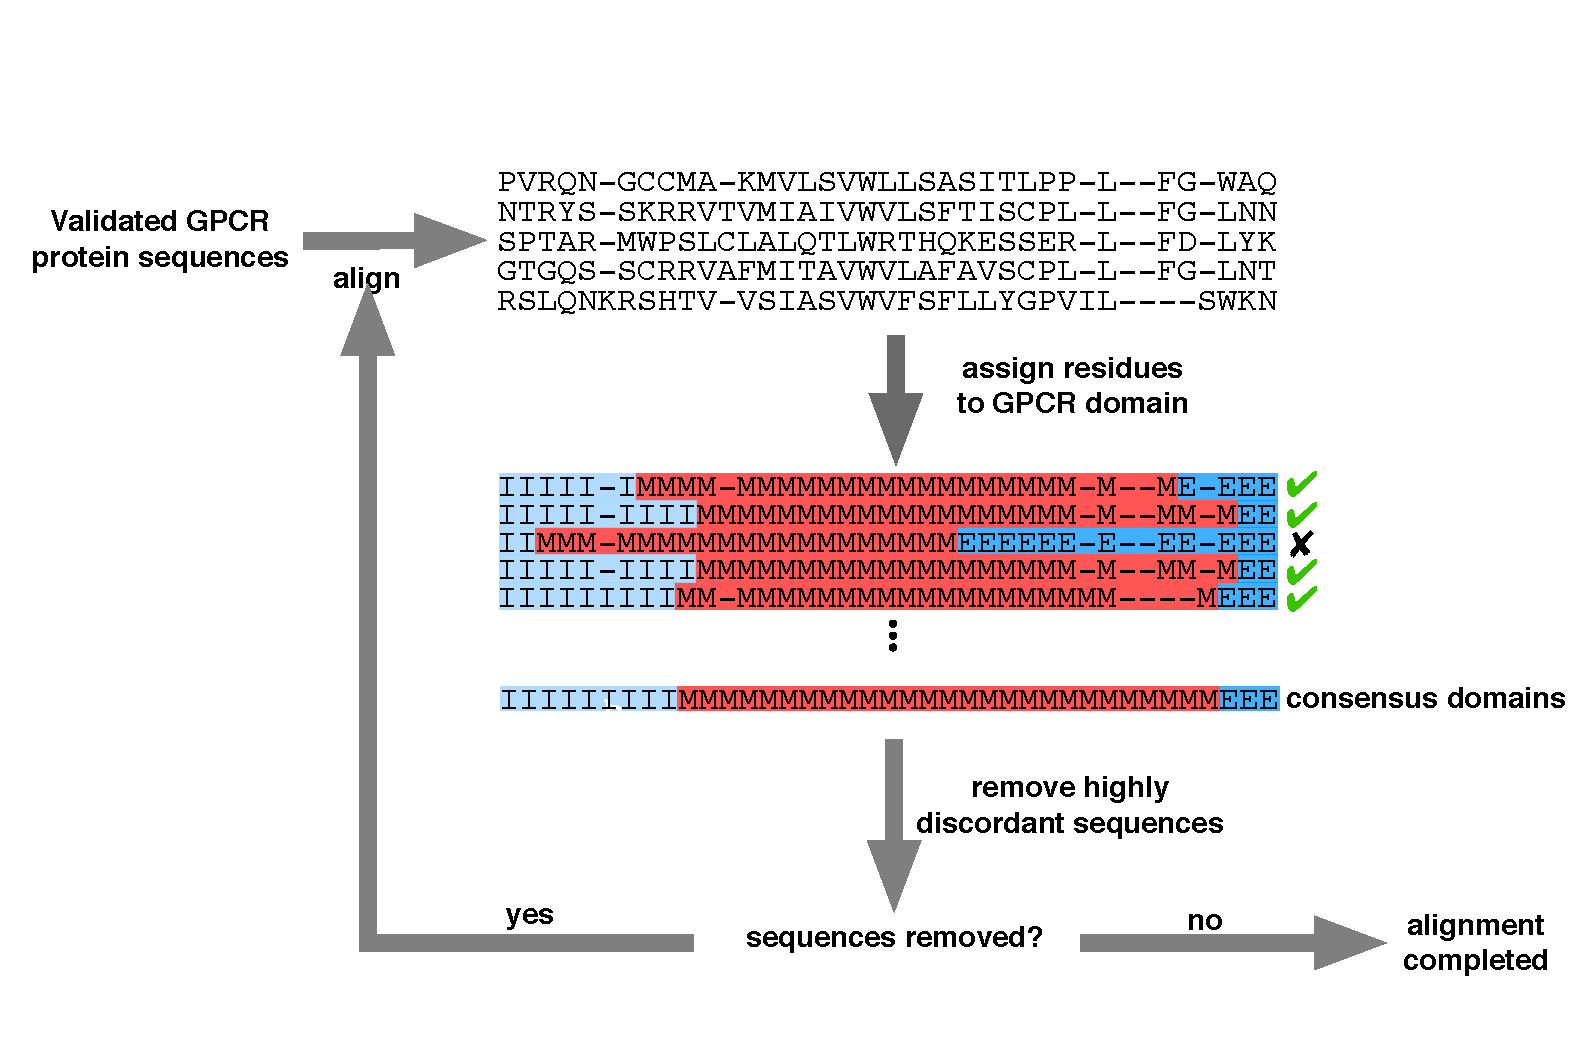
\includegraphics[width=18cm]{figures/alignment_flowchart.pdf}}
	\caption{\label{flowchart} Iterative alignment strategy to create a structurally-curated MSA of vertebrate biogenic amine receptors. A total of 3464 sequences were initially input (``Validated GPCR protein sequences''), and the final MSA contained 3039 protein sequences. Residues marked with ``I'' represent intracellular residues, those marked with ``M'' represent transmembrane residues, and those marked with ``E'' represent extracellular residues. MSA gaps were regarded as missing data when determining each column's consensus structural domain. Sequenced were removed (``remove highly discordant sequences'') if $\geq 5\%$ of columns belonged to a different structural domain than the respective consensus domain.}
\end{figure}


\newpage

\begin{figure}[htbp]
	\centerline{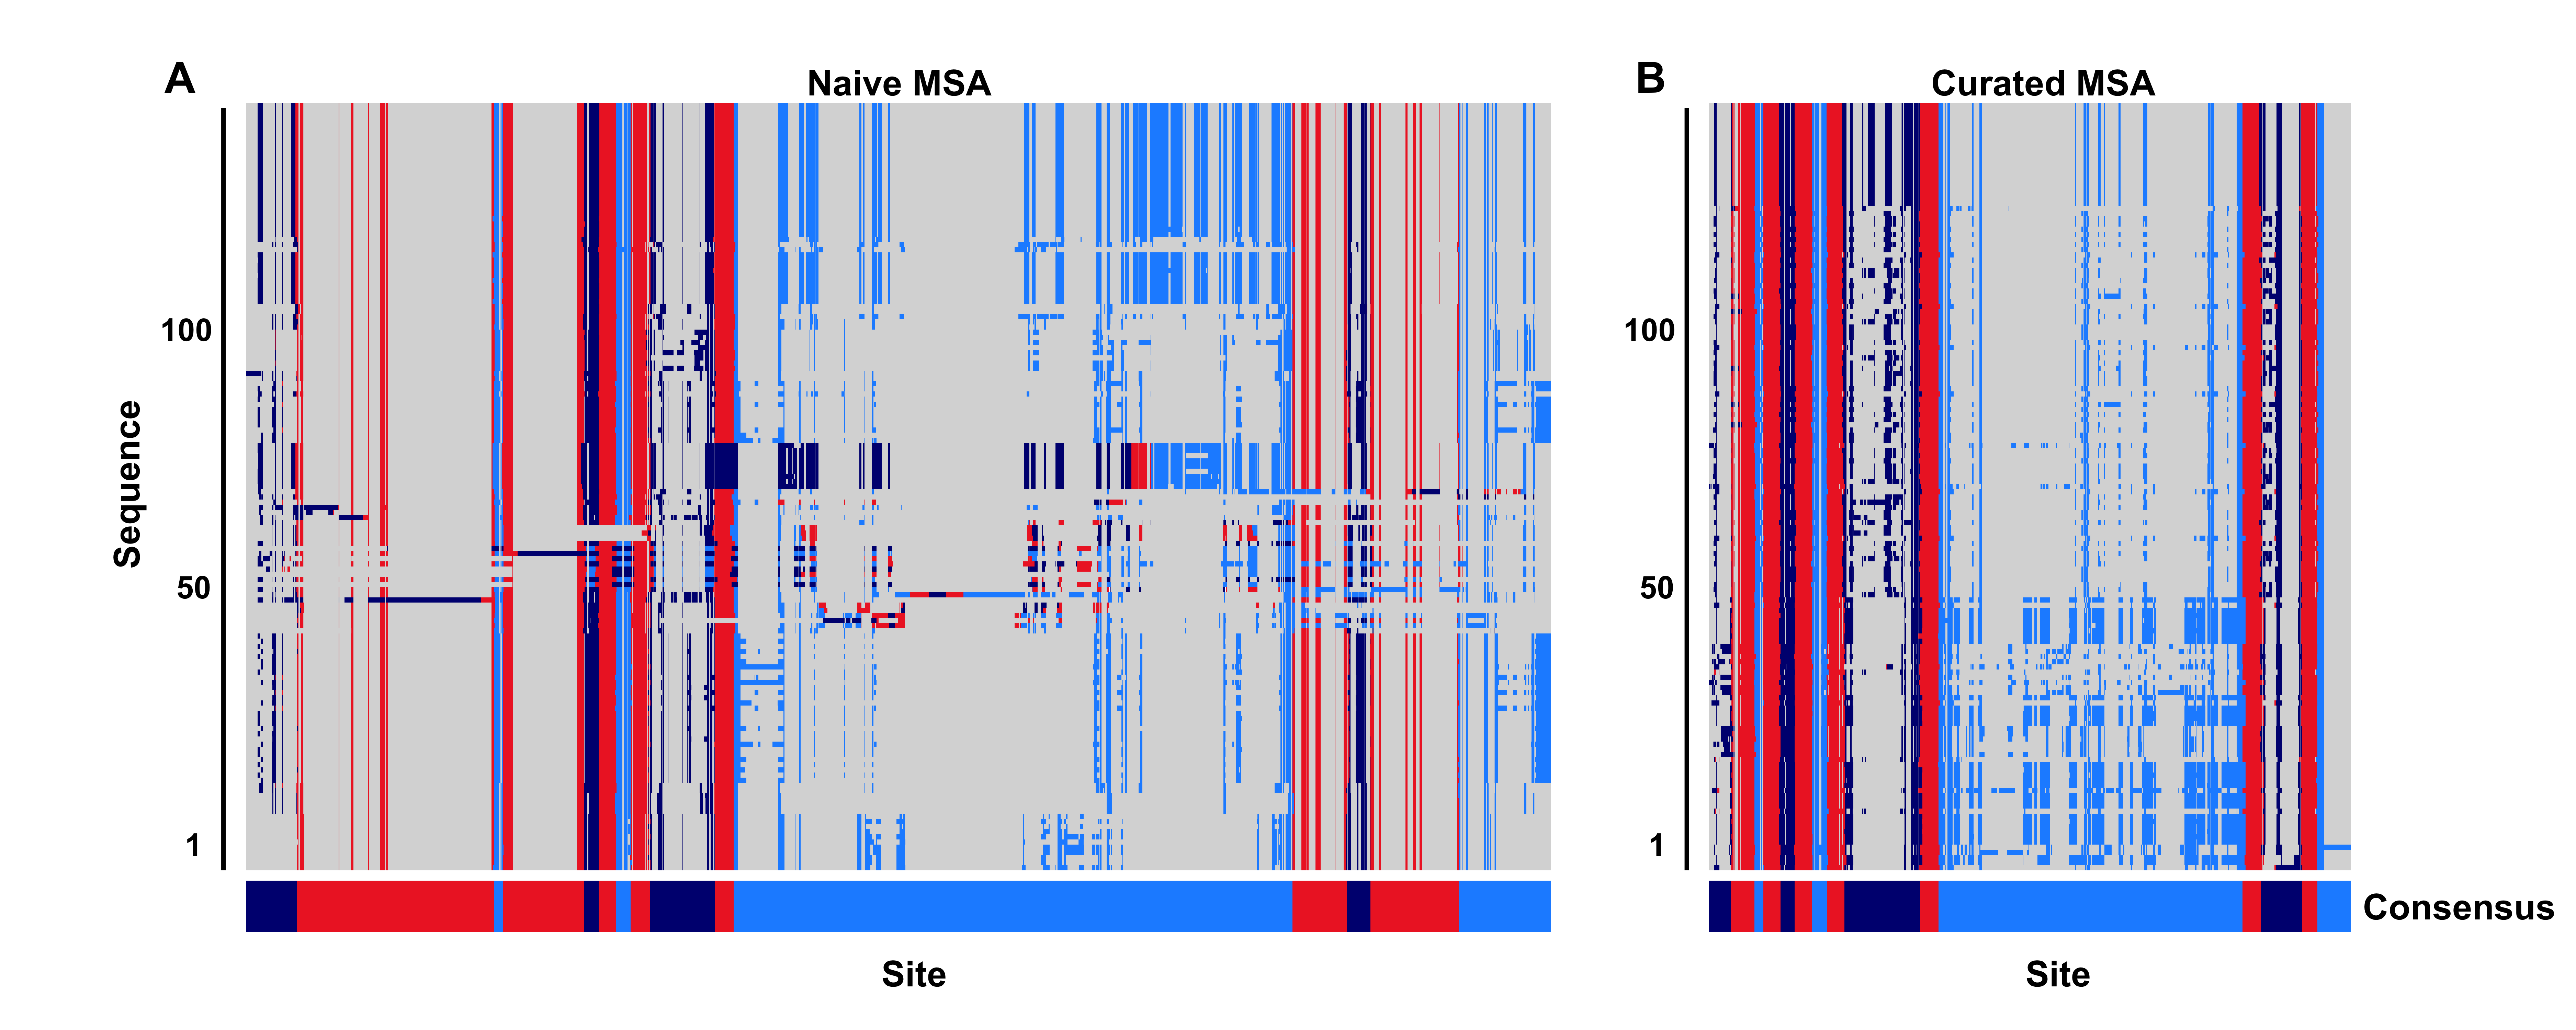
\includegraphics[width=6in]{figures/domains_naive_struc.png}}
	\caption{\label{domains} Graphical representation of a subset of the naive and structurally-curated biogenic amine receptor MSAs. Each image displays 130 MSA rows focused specifically on the MSA section containing the seven TM domains. Dark blue rectangles represent predicted extracellular residues, red rectangles represent predicted TM residues, lighter blue rectangles represent predicted intracellular residues, and gray represents MSA gaps. The bottom bar below each MSA figure shows the consensus domain structure. Note that all columns which contain only gaps in each MSA subset have been removed from this figure for visual clarity.}
\end{figure}


\vspace{3cm}

\begin{figure}[htbp]
	\centerline{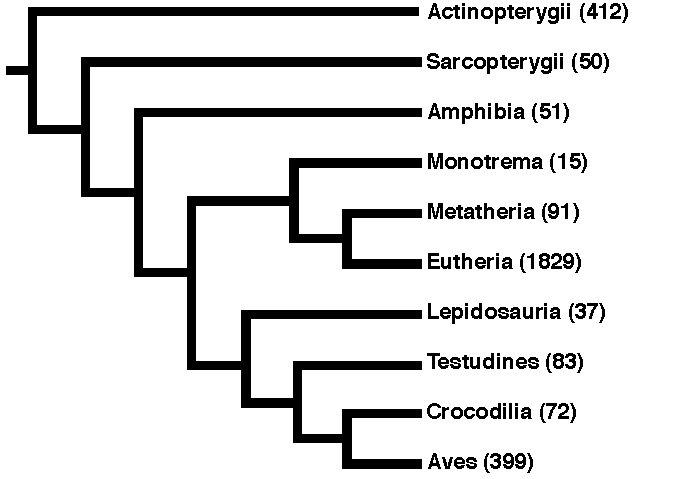
\includegraphics[width=7cm]{figures/taxonomic_distribution.pdf}}
	\caption{\label{taxa_dist} Cladogram of the taxonomic distribution of all sequences in the final structurally-curated MSA. All sequences belonged to the Euteleostomi clade of jawed vertebrates. Numbers in parentheses indicate the total number of sequences from the respective clade. We note that our MSA is particularly enriched for sequences from Eutherian (placental mammal) species, likely due to the stringent filters we applied to sequence collection that favored fully-sequenced genomes.}
\end{figure}

\vspace{3cm}

\begin{table}[htbp]
	\centering
	\begin{tabular}{l c l l c}
		\hline\noalign{\smallskip}
		\multicolumn{1}{c}{MSA} & \multicolumn{1}{c}{Partitioned} & \multicolumn{1}{c}{$\ln L$} & \multicolumn{1}{c}{k} & \multicolumn{1}{l}{$\Delta$AIC} \\
		\hline\noalign{\smallskip}
		Structural Masked & Yes & -505500.8 & 6115 & 0 \\
		Structural Masked & No & -515991.7 & 6095 & 1752 \\  
		Structural Unmasked & Yes & -515343.6 & 6115 & 19685 \\
		Structural Unmasked & No & -515991.7 & 6095 & 20941 \\ 
		Naive & No &  -589703.7 & 6945 & 170047 \\
		\noalign{\smallskip}\hline\noalign{\smallskip} 
	\end{tabular}
	\caption{\label{tab:phylo_AIC} $\Delta$AIC scores relative to the best performing for phylogenies. The column labeled ``Partitioned'' indicates whether phylogenetic inference was conducted with distinct TM (transmembrane) and EM (extramembrane) partitions. AIC is computed as AIC $= 2(k - \ln L)$, where $k$ is the number of free parameters of the model, and $\ln L$ is the log-likelihood \citep{Akaike1974,BurnhamAnderson2004}. AIC scores are reported here relative to the phylogeny with the lowest AIC score (structural masked with partitions), representing the best-fitting phylogeny.}
\end{table}


\newpage

\begin{figure}[htbp]
	\centerline{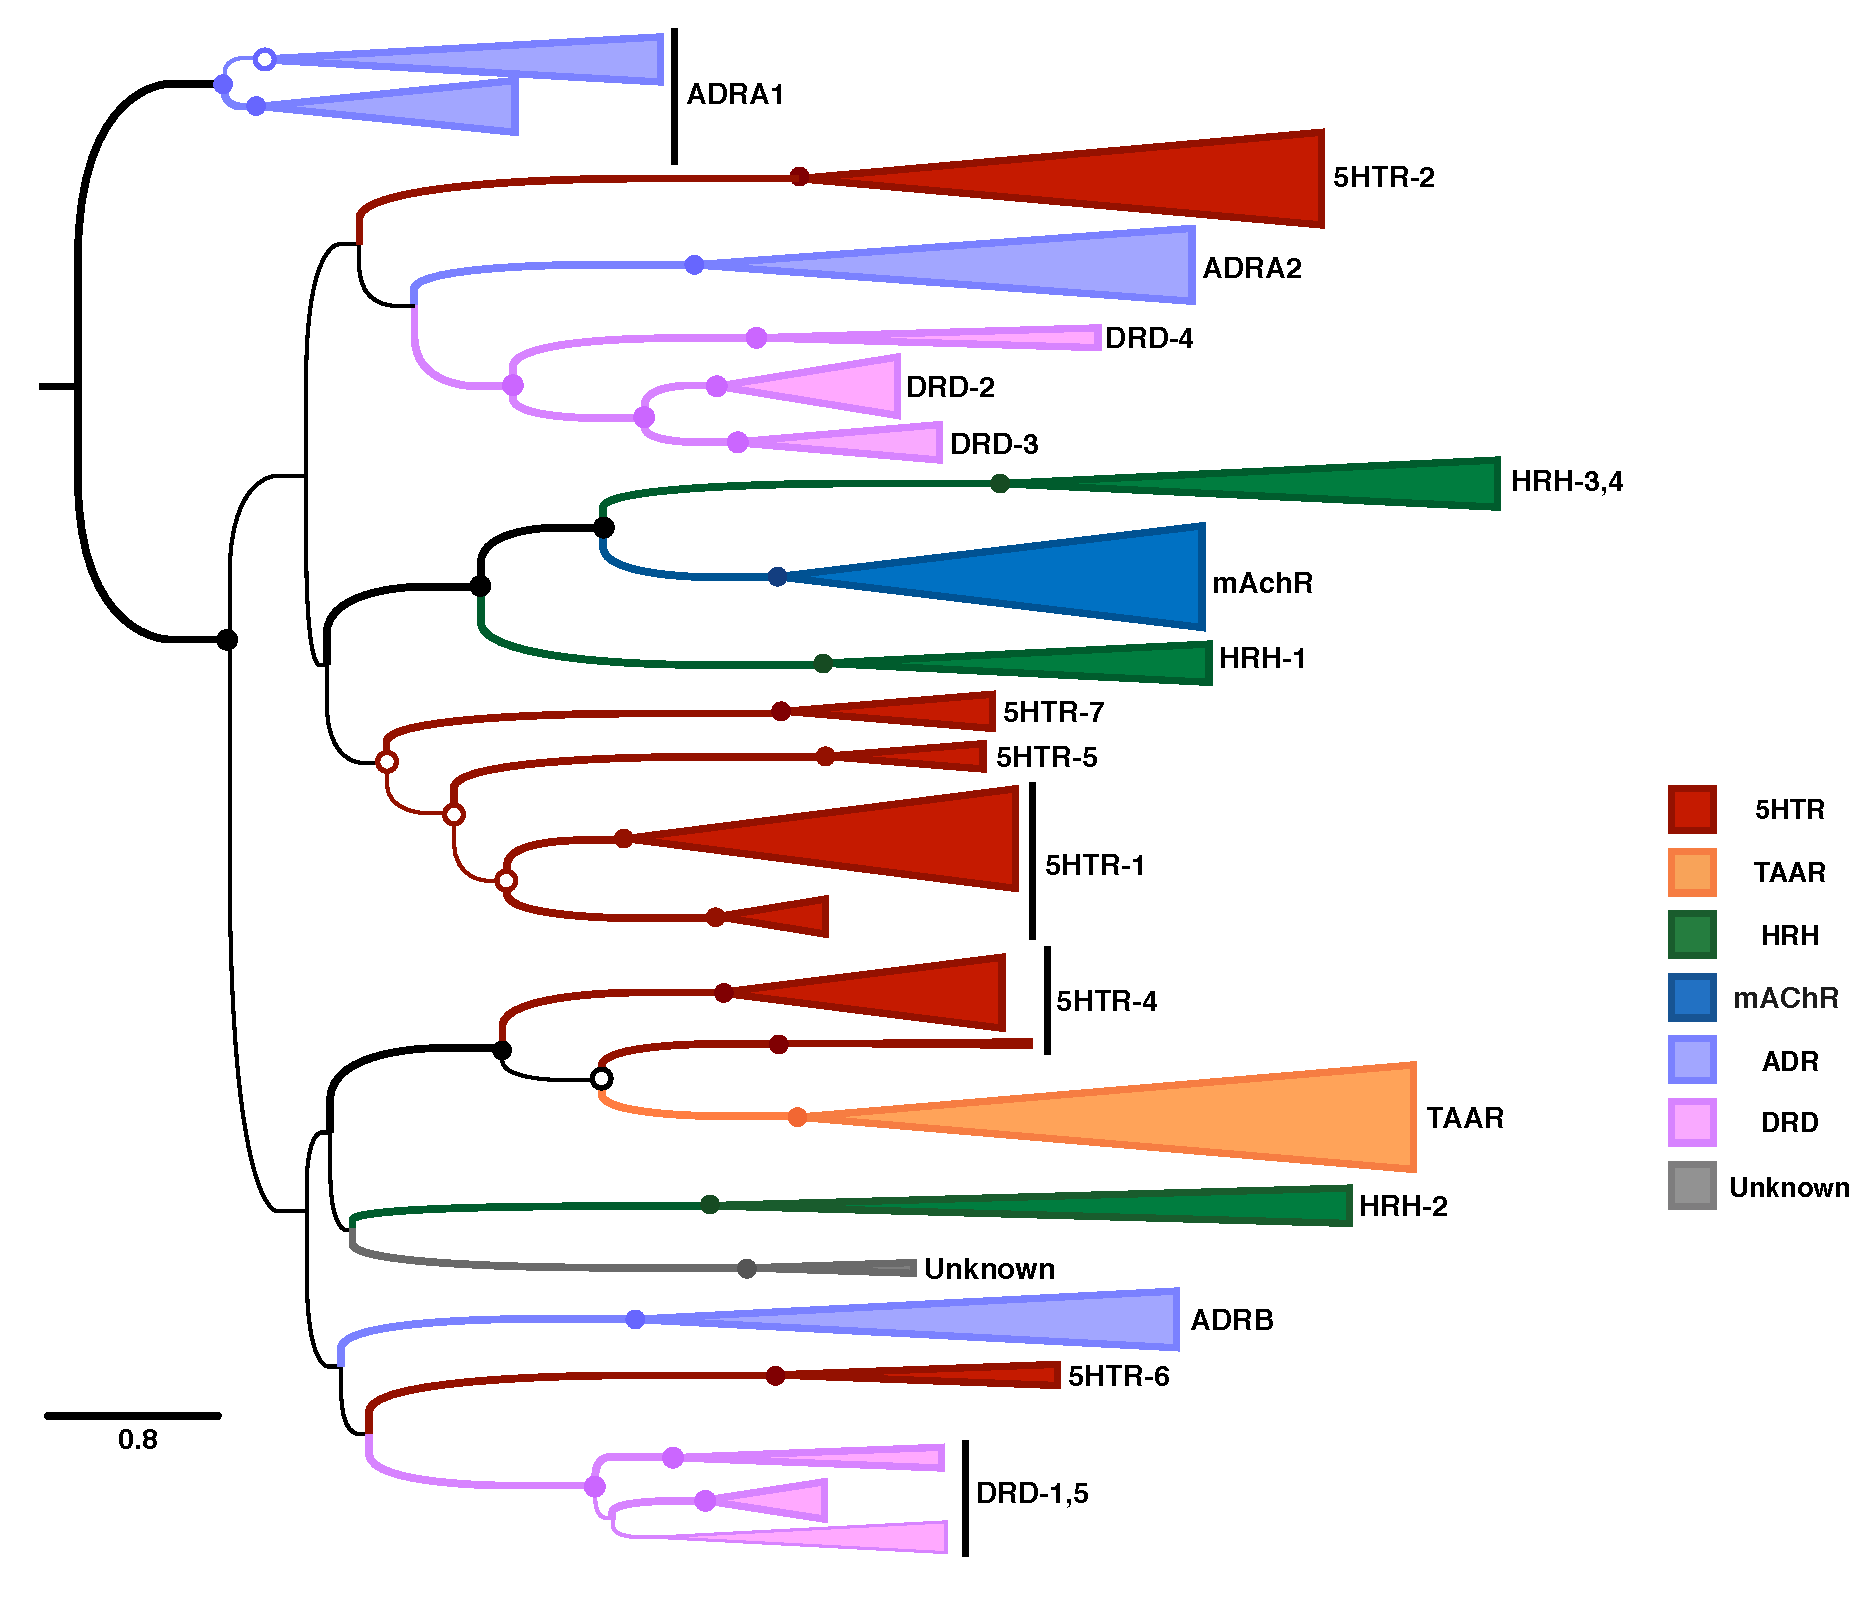
\includegraphics[width=18cm]{figures/masked_part_phylogeny.pdf}}
	\caption{\label{phylogeny} Maximum likelihood phylogeny of vertebrate biogenic amine receptors built using the masked structural MSA in RAxML. Nodes with open circles indicate $\geq 50\%$ bootstrap support, and nodes with closed circles and thick lines indicate $\geq 90\%$ bootstrap support. Biogenic amine receptors are abbreviated as 5HTR, serotonin receptors; TAAR, trace amine-associated receptors; HRH, histamine receptors; mAChr, muscarinic acetylcholine receptors; ADR, adreneric receptors; and DRD, dopamine receptors. The clade labeled ``Unknown'' could not be clearly identified as one of the major receptor types and may represent a novel biogenic amine receptor clade.}
\end{figure}


\newpage

\begin{figure}[htbp]
	\centerline{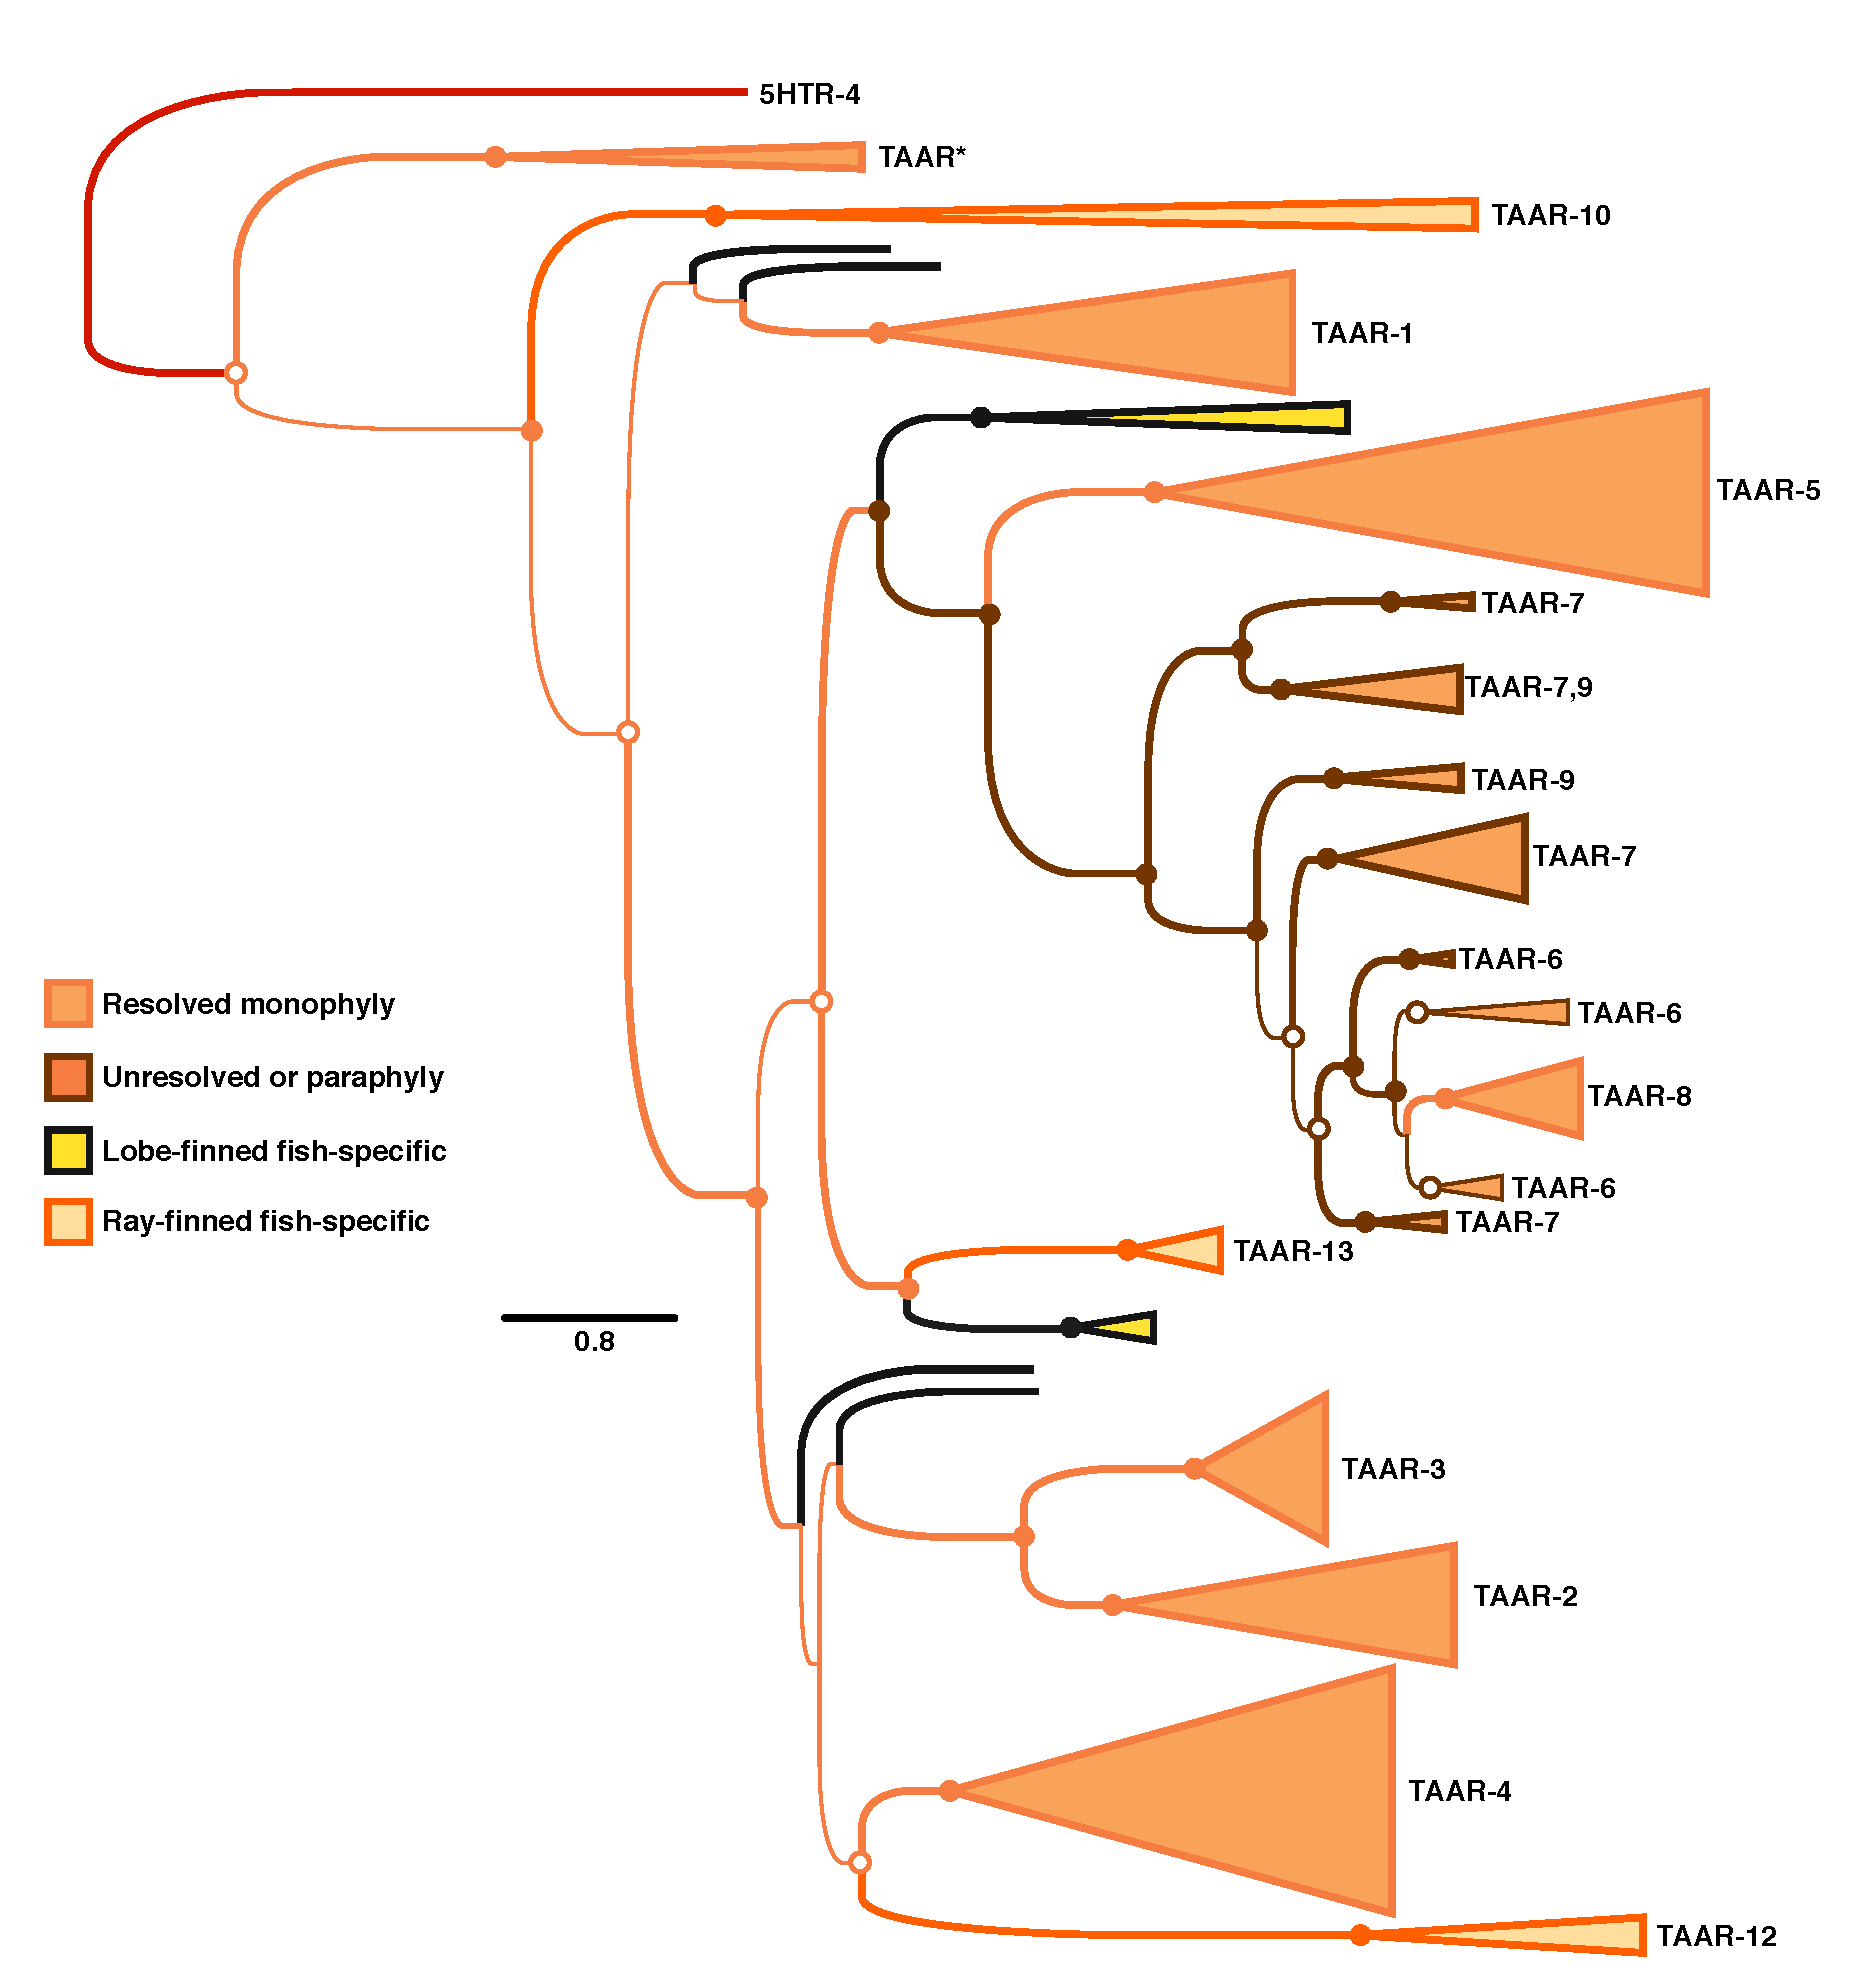
\includegraphics[width=15cm]{figures/taar_phylogeny.pdf}}
	\caption{\label{taar_tree} Subclade of the TAAR receptors within the phylogeny shown in Figure~\ref{phylogeny}. Nodes with open circles indicate $\geq 50\%$ bootstrap support, and nodes with closed circles and thick lines indicate $\geq 90\%$ bootstrap support.}
\end{figure}


% % % % % % % % % % % %    OVERFLOW    % % % % % % % % % % % % % %
%Alternatively, we suggest that filtering our naive MSA based on uncertainty measures would not necessarily have improved MSA quality. Indeed, filtering unreliable MSA columns and/or residues from the naive MSA would not have addressed the true underlying problem: inappropriately aligned \emph{sequences} forced inappropriate gaps into the MSA. Thus, the primary issue with the naive MSA was that certain sequences did  
%The main problem in our naive MSA, on the other hand, was the presence of confounding sequences that did not properly align to the overarching structure and thus forced inappropriate gaps into the MSA.  
%not have resolved the majority of problems in the MSA. Indeed, MSA uncertainty arises primarily in highly-gapped MSA regions, yet gaps were not necessarily a problem in our MSA. In fact, the extreme length variability across GPCR terminal and loop domains necessitates a fair number of gaps. Using an algorithm that removes gappy MSA regions, such as Gblocks \citep{Castresana2000}, would not remove this underlying issue, as the improperly aligned sequences would remain in the MSA. Instead, only by removing entire sequences were we able to alleviate MSA concerns to achieve a comprehensive, structurally-curated MSA. 






\end{document}